\chapter{Comportamiento dinámico y estabilidad}
El concepto de estabilidad y su análisis constituye unos de los aspectos claves para el estudio de los sistemas dinámicos. La estabilidad de un sistema esta estrechamente relacionada con su comportamiento dinámico y puede definirse de diversas maneras. En este capítulo nos centraremos en el análisis de los llamados puntos de equilibrio de un sistema y los estudiaremos de acuerdo con el concepto de estabilidad de Lyapunov. Además, incidiremos en otros aspectos de la estabilidad de los sistemas tales como la existencia de ciclos límite o el movimiento nominal. Empecemos pues por el estudio de los puntos de equilibrio.

\section{Sistemas autónomos}

\subsection{Puntos de equilibrio} 
\begin{definition}[Punto de equlibrio] Dados un sistema dinámico general definido por las ecuaciones,
\begin{align}
\mathbf{\dot{x}} = \mathbf{f}(\mathbf{x},\mathbf{u})\\
\mathbf{y} = \mathbf{g}(\mathbf{x},\mathbf{u})
\end{align}
donde $\mathbf{x} \in \mathbb{R}^n$, $\mathbf{u} \in \mathbb{R}^m$ e $\mathbf{y} \in \mathbb{R}^l$. Se definen como puntos de equilibrio o puntos estacionarios los valores del vector de estados $\mathbf{x_e}$ y del vector de entradas $\mathbf{u_e}$ para los cuales el estado y, consecuentemente, la salida del sistema permanecen constantes,

\begin{align}
\mathbf{\dot{x}_e} \equiv 0 = \mathbf{f}(\mathbf{x_e},\mathbf{u_e})\\
\mathbf{y_e} = \mathbf{g}(\mathbf{x_e},\mathbf{u_e})
\end{align}
\end{definition}

Si el vector de estados no cambia, su derivada será cero. Por tanto, mientras no se altere el valor de la entrada, el sistema permanecerá en el mismo estado y el valor del vector de salidas permanecerá también constante

Podemos, a partir de esta definición, obtener algunas propiedades importantes de los puntos de equilibrio:
\begin{enumerate}
\item Una vez que un sistema alcanza un punto de equilibrio, permanece en él indefinidamente. (Todas las derivadas temporales de las componentes del vector de estado son cero.
\item Desde el punto de vista del control de sistemas, los puntos de equilibrio juegan un papel importante ya que representan condiciones de operación constante.
\item Un sistema dinámico puede tener uno o más puntos de equilibrio, o no tener ninguno. 
\end{enumerate}

\paragraph{Sistemas autónomos.} Para simplificar el estudio de la estabilidad, podemos empezar por considerar el casos de sistemas que tienen entrada nula $\mathbf{u} = \mathbf{0}, \ \forall t$. en los que la entrada es una función directa de los estados del sistema. Hablaremos entonces de un \emph{sistema autónomo}; la salida evoluciona a partir de un estado inicial $\mathbf{x_0}\equiv \mathbf{x(t_0)}$,

\begin{align}
\mathbf{\dot{x}} = \mathbf{f}(\mathbf{x})\\
\mathbf{y} = \mathbf{g}(\mathbf{x})
\end{align}

\paragraph{Sistemas realimentados.} Del mismo modo, podemos considerar sistemas en los que la entrada es una función directa del valor de los estados; $\textbf{u}= \textbf{c(x)}$. Hablaremos entonces de un \emph{sistema realimentado}. A efectos de análisis de la estabilidad del sistema, no hay diferencia entre un sistema realimentado y un sistema autónomo,
\begin{align}
\mathbf{\dot{x}} = \mathbf{f}(\mathbf{x},\mathbf{c(x)}) = \bar{f}(\mathbf{x})\\
\mathbf{y} = \mathbf{g}(\mathbf{x},\mathbf{c(x)}) = \bar{\mathbf{g}}(\mathbf{x})
\end{align}
El nombre de sistema realimentado, proviene de considerar que se están \emph{realimentando} los estados en la entrada del sistema. El concepto de realimentación constituye uno de los pilares de los sistemas de control. La figura \ref{fig:rea}, muestra esquemáticamente este concepto.

\begin{figure}
\centering
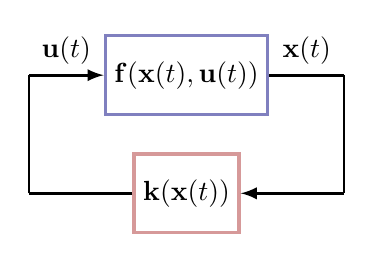
\begin{tikzpicture}
\draw(0,0) node(p)[rectangle, minimum height=10mm, minimum width=10mm,align=center, very thick, draw = blue!50!black!50]{$\mathbf{f}(\mathbf{x}(t),\mathbf{u}(t))$}

(0,-1.5) node(c)[rectangle, minimum height=10mm, minimum width=10mm,align=center ,very thick,draw = red!60!black!40]{$\mathbf{k}(\mathbf{x}(t))$};

\draw[line width = 1pt](p)--(2,0)node[midway,above]{$\mathbf{x}(t)$};
\draw[line width = 1pt](2,0)--(2,-1.5);
\draw[line width = 1pt, -latex](2,-1.5)--(c);
\draw[line width = 1pt](c)--(-2,-1.5);
\draw[line width = 1pt](-2,-1.5)--(-2,0);
\draw[line width = 1pt, -latex](-2,0)--(p)node[midway,above]{$\mathbf{u}(t)$};

\end{tikzpicture}

\caption{Esquema general de un sistema realimentado}\label{fig:rea}
\end{figure}

Tanto para un sistema autónomo como para uno realimentado los puntos de equilibrio deberán satisfacer la condición de que las derivadas temporales de los estados sean todas nulas,
\begin{equation}
\mathbf{0} = \mathbf{f(x_e})
\end{equation}

\section{Estabilidad de Lyapunov}
La teoría de la estabilidad constituye un aspecto importante dentro del estudio de los sistemas dinámicos. Puede abordarse desde diversos puntos de vista. En esta sección vamos a centrarnos en el estudio de la estabilidad de los puntos de equilibrio. 

Habitualmente, cuando se trata de la estabilidad de los puntos de equilibrio se suele hablar de estabilidad en el \emph{sentido} de Lyapunov. Aleksandr Mikhailovich Lyapunov un matématico ruso, de finales del siglo XIX, que estableció los fundamentos de la teoría de la estabilidad que ahora lleva su nombre.

Un punto de equilibrio de un sistema dinámico es \emph{estable} si toda  solución que comienzan cerca del punto de equilibrio permanece cercana al punto de equilibrio; en otro caso, el punto de equilibrio es inestable. Es \emph{asintóticamente estable} si toda solución que empieza próxima al punto de equilibrio no solo permanecen cerca del punto de equilibrio sino que tienden a él cuando el tiempo tiende a infinito.

\subsection{Estabilidad de Lyapunov para sistemas autónomos}
Consideremos un sistema autónomo genérico,
\begin{equation}\label{eq: aut}
\dot x = f(x),
\end{equation}
donde $f(x): D\rightarrow \mathbb{R}^n$ es una función (localmente) lipschitziana desde un domino $D \subset \mathbb{R}^n$ a $\mathbb{R}^n$. Supongamos además que $\overline x \in D$ es un punto de equilibrio; es decir, $f(\overline x) = 0$. Lo que buscamos es un método para caracterizar el tipo de estabilidad de $\overline x$. En lo que sigue, y sin perdida de generalidad, consideramos que el punto de equilibrio es es origen de coordenadas $\overline x = 0$ \footnote{Siempre es posible hacer un cambio de coordenadas de modo que si $\overline x \neq 0$, $z = x-\overline x$; $\dot z = \dot x = f(x+\overline x) := g(z)$, donde $g(0)=0$.}.

\begin{definition}
El punto de equilibrio x = 0 del sistema \ref{eq: aut} es:
\begin{itemize}
\item estable $\forall \epsilon > 0$ que cumpla:
\begin{equation*}
 \exists \delta =\delta(\epsilon)>0: \| x(0) \| < \delta \Rightarrow \| x(t)\| < \epsilon \ \forall t \ge 0
\end{equation*}
 
 \item Es inestable si no es estable.
 \item Es asintóticamente estable si es estable y además se puede elegir $delta$ de modo que,
\begin{equation*}
\| x(0)\| < \delta \Leftarrow \lim_{t \to \infty} x(t) = 0
\end{equation*}
\end{itemize}
\end{definition}

En 1892 Lyaponov propuso un método para analizar la estabilidad de un punto de equilibrio, basado en el análisis  una función $V:D\to \mathbb{R}$, continua y diferenciable en un entorno $D \subset \mathbb{R}^n$. En concreto, el método analiza la variación de la función $V$ a lo largo de las \emph{trayectorias} del sistema cuya estabilidad se quiere analizar, Podemos representar dicha variación empleando la derivada temporal de la función $V$
\begin{equation}
\dot V(x) = \sum_{i=0}^{n}\frac{\partial V}{\partial x_i} \dot x_i = \sum_{i=0}^{n}\frac{\partial V}{\partial x_i} f(x) = \frac{\partial V}{\partial x}f(x)
\end{equation}

Es interesante hacer notar que, lógicamente, $dot V$ depende del sistema que se desea analizar y que Si $\phi(t;x)$ es una solución del sistema \ref{eq: aut} que tiene como condición inicial estado $x$, para $t=0$ Entonces,
\begin{equation}
\dot V(x) =\left. \frac{d}{dt}V(\phi (t;x))\right|_{t=0}
\end{equation}
\section{Principio de invarianza de LaSalle}

